\chapter{Fondements théoriques des convertisseurs temps-numérique}
\label{chap:tdc-fondements}
\justifying
\sloppy

\section{Rôle d'un TDC dans une chaîne de détection}

Un convertisseur temps-numérique a pour fonction de transformer un intervalle de temps en un mot binaire exploitable par une chaîne numérique. Cette opération est indispensable dès lors que l'information utile n'est pas portée uniquement par l'amplitude d'un signal, mais aussi par son instant d'apparition, sa durée, ou le décalage temporel entre deux événements. Dans le domaine de l'instrumentation scientifique, cette capacité intervient notamment pour la chronométrie fine, la localisation temporelle d'un événement et l'amélioration de la reconstruction globale d'un système de détection \cite{annagrebah2021thesis,henzler2010tdc}.

Dans sa forme la plus générale, un \textbf{TDC} reçoit deux événements : un événement de départ, qui initialise l'observation, puis un événement d'arrêt, qui ferme l'intervalle à mesurer. Dans une architecture intégrée réelle, cette vision simplifiée doit être enrichie : les événements sont asynchrones, la conversion peut produire plusieurs détections associées à un même intervalle, la fermeture peut aussi être déclenchée par un watchdog, et la valeur exportée n'est pas toujours un horodatage final prêt à l'emploi. Dans de nombreuses architectures modernes, le \textbf{TDC} fournit plutôt un ensemble d'observables qui devront ensuite être interprétées, corrigées et parfois recalibrées.

La figure \ref{fig:tdc-measurement-chain} résume cette idée à l'échelle système. Elle donne volontairement une vue d'ensemble avant de zoomer, dans les chapitres suivants, sur le mécanisme Vernier puis sur l'architecture qui l'exploite. Une chaîne de lecture dédiée à la mesure du temps comprend généralement un détecteur ou une source d'événement, une interface d'entrée chargée de mettre le signal en forme, puis un \textbf{TDC} responsable de la conversion de l'information temporelle en données numériques.

\begin{figure}[H]
    \centering
    
\includegraphics[width=0.92\textwidth]{tdc/tdc_measurement_chain.pdf}
    \caption{Schéma de synthèse d'une chaîne de mesure temporelle, du détecteur au codage binaire.}
    \label{fig:tdc-measurement-chain}
\end{figure}

Dans \textbf{SPADMIC}, cette chaîne de mesure doit rester compatible avec des événements asynchrones, un format de sortie compact et une correction externe. Les contraintes fondamentales sont donc moins celles d'un \textbf{TDC} isolé que celles d'un bloc de mesure intégré dans une chaîne de lecture complète.

\section{Grandeurs de performance à considérer}

L'analyse d'un \textbf{TDC} ne se limite pas à sa seule résolution nominale. Plusieurs métriques complémentaires sont nécessaires pour caractériser son comportement \cite{annagrebah2021thesis}. Dans un projet comme \textbf{SPADMIC}, cette lecture multi-critère est indispensable, car une amélioration d'une grandeur peut dégrader fortement une autre.

\subsection{Résolution temporelle et plage dynamique}

La première métrique est la résolution temporelle, souvent notée $T_{\mathrm{LSB}}$. Elle correspond au plus petit intervalle de temps que le convertisseur peut discriminer. Dans un convertisseur idéal, cette grandeur joue un rôle analogue au bit de poids faible d'un convertisseur analogique-numérique. Dans la pratique, cette grandeur ne doit pas être confondue avec la précision mesurée en \textbf{RMS} : une résolution nominale très fine ne garantit pas, à elle seule, une dispersion faible.

La seconde métrique est la plage dynamique. Elle désigne l'intervalle maximal que le convertisseur peut mesurer tout en conservant un codage exploitable. En pratique, une architecture très précise mais de faible dynamique devient rapidement difficile à utiliser si elle ne couvre pas les délais réellement rencontrés dans le système. Dans un \textbf{Vernier} à oscillateurs en anneau, cette dynamique dépend non seulement de la profondeur disponible du compteur grossier, mais aussi du temps nécessaire au rattrapage entre oscillateur lent et oscillateur rapide.

\subsection{Résolution effective temporelle}

Par analogie avec la définition de l'\textbf{ENOB} utilisée pour les convertisseurs analogique-numérique, on peut définir un indicateur temporel effectif adapté au \textbf{TDC} \cite{ieee1241_2010}. Cette grandeur ne remplace pas les métriques de résolution, de \textbf{DNL}, d'\textbf{INL} ou d'erreur \textbf{RMS}, mais elle permet de résumer le nombre de bits réellement exploitables sur une plage temporelle donnée. Si $T_{\mathrm{FS}}$ désigne la plage temporelle couverte et $\sigma_e$ l'erreur temporelle \textbf{RMS} effective, une écriture usuelle consiste à poser :
\[
    ENOB_{\mathrm{TDC}} = \log_2\left(\frac{T_{\mathrm{FS}}}{\sqrt{12}\,\sigma_e}\right).
\]
La plage $T_{\mathrm{FS}}$ dépend notamment de la profondeur disponible du compteur grossier, tandis que $\sigma_e$ regroupe les contributions de quantification, de non-linéarité, de jitter et de calibration résiduelle. Cette métrique doit donc être interprétée comme un indicateur synthétique, et non comme une preuve suffisante de performance.

\subsection{Linéarité}

La linéarité traduit l'écart entre la caractéristique réelle du convertisseur et sa caractéristique idéale. Deux indicateurs sont classiquement utilisés \cite{annagrebah2021thesis,kalisz2004review} :
\begin{itemize}
    \item la non-linéarité différentielle (\textbf{DNL}), qui mesure l’écart de largeur d’un palier par rapport à $1$~LSB ;
    \item la non-linéarité intégrale (\textbf{INL}), qui cumule ces écarts le long de la fonction de transfert.
\end{itemize}

La DNL peut être comprise visuellement comme l'écart entre la largeur réelle d'un palier de la fonction de transfert et la largeur idéale de $1$~LSB.
\begin{figure}[H]
    \centering
    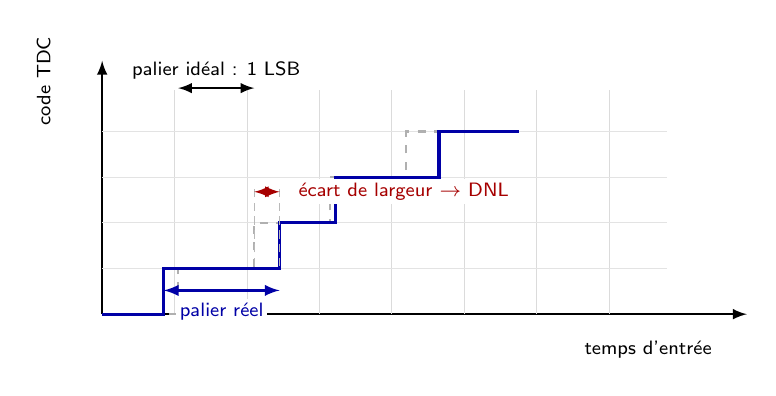
\begin{tikzpicture}[x=0.92cm,y=0.58cm,>=latex]
        \tikzset{
            axislabel/.style={font=\sffamily\scriptsize},
            annot/.style={font=\sffamily\scriptsize,fill=white,inner sep=1.4pt,align=center}
        }

        \draw[->,line width=0.75pt] (0,0) -- (8.9,0);
        \node[axislabel,anchor=north east] at (8.55,-0.38) {temps d'entrée};
        \draw[->,line width=0.75pt] (0,0) -- (0,5.55);
        \node[axislabel,anchor=south,rotate=90] at (-0.58,5.1) {code TDC};

        \foreach \x in {1,2,3,4,5,6,7} {
            \draw[gray!28,line width=0.3pt] (\x,0) -- (\x,4.9);
        }
        \foreach \y in {1,2,3,4} {
            \draw[gray!22,line width=0.3pt] (0,\y) -- (7.8,\y);
        }

        \draw[gray!62,dashed,line width=0.75pt]
            (0,0) -- (1.05,0) -- (1.05,1) -- (2.1,1) -- (2.1,2) -- (3.15,2)
            -- (3.15,3) -- (4.2,3) -- (4.2,4) -- (5.25,4);

        \draw[blue!65!black,line width=1.2pt]
            (0,0) -- (0.85,0) -- (0.85,1) -- (2.45,1) -- (2.45,2)
            -- (3.22,2) -- (3.22,3) -- (4.65,3) -- (4.65,4) -- (5.75,4);

        \draw[<->,line width=0.7pt] (1.05,4.95) -- (2.1,4.95);
        \node[annot,anchor=south] at (1.575,5.04) {palier idéal : 1 LSB};

        \draw[<->,blue!65!black,line width=0.85pt] (0.85,0.52) -- (2.45,0.52);
        \node[annot,text=blue!65!black,anchor=north] at (1.65,0.34) {palier réel};

        \draw[gray!55,densely dashed,line width=0.55pt] (2.1,1.05) -- (2.1,2.85);
        \draw[gray!55,densely dashed,line width=0.55pt] (2.45,1.05) -- (2.45,2.85);
        \draw[<->,red!65!black,line width=0.8pt] (2.1,2.68) -- (2.45,2.68);
        \node[annot,text=red!65!black,anchor=west] at (2.65,2.68) {écart de largeur $\rightarrow$ DNL};
    \end{tikzpicture}
    \caption{Illustration qualitative de la DNL sur une fonction de transfert de TDC. Un palier dont la largeur temporelle diffère de $1$~LSB contribue à la non-linéarité différentielle.}
    \label{fig:dnl-inl-tdc-step}
\end{figure}

Les expressions usuelles de la DNL et de l'INL s'écrivent alors :
\begin{equation}
    \mathrm{DNL}(n)=\frac{\Delta T_{n+1,n}-T_{\mathrm{LSB}}}{T_{\mathrm{LSB}}}
\end{equation}

\begin{equation}
    \mathrm{INL}(i)=\sum_{n=1}^{i}\mathrm{DNL}(n)
\end{equation}

Une bonne résolution ne suffit donc pas. Un convertisseur réellement exploitable doit également conserver une linéarité compatible avec la précision recherchée.

\subsection{Précision temporelle RMS}

Une autre métrique essentielle est l'erreur de conversion exprimée sous forme \textbf{RMS}. Elle reflète la dispersion de l'erreur lorsque le convertisseur est soumis aux différentes sources d'aléas : bruit électronique, jitter, bruit de quantification ou variations des conditions opératoires. Pour un \textbf{TDC} Vernier, cette grandeur constitue un indicateur central de la précision temporelle effective \cite{annagrebah2021thesis}, particulièrement sensible au jitter cumulé des oscillateurs et à la façon dont la frontière grossière/fine est reconstruite.

\subsection{Temps mort, débit et observabilité}

Dans une architecture embarquée, il faut également considérer le temps mort et le débit. Le temps mort représente l'intervalle minimal entre deux mesures acceptées. Il dépend de la fermeture de la conversion, du nettoyage interne des détecteurs de phase, de la remise à zéro des compteurs et du mécanisme de réarmement. Le débit, lui, dépend en plus de la lecture, de la profondeur des files FIFO et de la présence éventuelle de rétropression sur la sortie numérique.

Enfin, l'observabilité constitue une métrique moins classique mais essentielle pour l'architecture visée. Un \textbf{TDC} qui n'exporte qu'un code final compact peut être suffisant dans un cas d'usage simple, mais il devient difficile à recalibrer, à diagnostiquer ou à caractériser finement. À l'inverse, un bloc qui exporte des observables riches permet un traitement externe à l'ASIC plus puissant, au prix d'un format de sortie plus élaboré.

\section{Panorama des grandes familles d'architectures}

La littérature distingue plusieurs familles d'architectures pour la mesure d'intervalles de temps \cite{annagrebah2021thesis,henzler2010tdc}. Parmi les plus importantes, on retrouve :
\begin{itemize}
    \item les architectures analogiques de type \textbf{TAC}, qui convertissent le temps en tension avant numérisation ;
    \item les architectures numériques à \textbf{compteur}, très intégrables mais limitées par la fréquence d’horloge requise pour atteindre de très fines résolutions ;
    \item les structures à \textbf{ligne à délais}, qui exploitent les retards élémentaires des cellules logiques ;
    \item les architectures à \textbf{oscillateurs en anneau}, intéressantes pour combiner compacité et dynamique ;
    \item les architectures \textbf{Vernier}, qui exploitent la différence entre deux délais ou deux périodes proches pour descendre sous le seuil technologique imposé par un seul élément de retard.
\end{itemize}

Le tableau \ref{tab:tdc-arch-compare} synthétise les compromis les plus importants. Les ordres de grandeur indiqués sont volontairement donnés à titre comparatif : ils dépendent fortement de la technologie, du niveau d'intégration et des choix d'implémentation. Ils restent néanmoins suffisants pour motiver le choix architectural retenu dans \textbf{SPADMIC}.

\begin{table}[H]
    \centering
    \small
    \begin{tabularx}{\textwidth}{>{\raggedright\arraybackslash}p{2.5cm}>{\raggedright\arraybackslash}X>{\raggedright\arraybackslash}p{2cm}>{\raggedright\arraybackslash}p{1.9cm}>{\raggedright\arraybackslash}p{1.6cm}>{\raggedright\arraybackslash}p{1.6cm}}
        \toprule
        \textbf{Architecture} & \textbf{Principe} & \textbf{Résolution typique} & \textbf{Plage dynamique} & \textbf{Surface} & \textbf{Puissance} \\
        \midrule
        TAC analogique & Intégration d'un courant sur condensateur puis conversion ADC & \SIrange{10}{100}{\pico\second} & Moyenne & Moyenne & Moyenne à élevée \\
        Compteur numérique & Horloge de référence échantillonnée au \texttt{START}/\texttt{STOP} & $>\SI{100}{\pico\second}$ sauf horloge très rapide & Très large & Faible & Forte si l'horloge monte en fréquence \\
        Ligne à délais & Propagation d'une impulsion le long d'une chaîne de retard & \SIrange{10}{100}{\pico\second} & Courte à moyenne & Élevée si la plage augmente & Faible à moyenne \\
        DLL / PLL / interpolation & Phases verrouillées ou interpolation fractionnaire & \SIrange{5}{20}{\pico\second} & Moyenne & Moyenne à élevée & Moyenne à élevée \\
        Oscillateur en anneau & Comptage sur oscillateur local et capture de phase & \SIrange{20}{100}{\pico\second} & Moyenne à large & Faible à moyenne & Moyenne \\
        Vernier ligne à délais & Deux chaînes à retards légèrement différents & \SIrange{1}{20}{\pico\second} & Moyenne & Élevée & Moyenne \\
        Vernier RO multiphase & Deux oscillateurs + observation multiphase des croisements & \SIrange{5}{20}{\pico\second} nominal brut & Moyenne à large & Moyenne & Moyenne \\
        \bottomrule
    \end{tabularx}
    \caption{Comparaison synthétique des principales familles de \textbf{TDC}. Les ordres de grandeur sont indicatifs et servent ici à positionner le compromis recherché pour \textbf{SPADMIC} \cite{annagrebah2021thesis}.}
    \label{tab:tdc-arch-compare}
\end{table}

\section{Pourquoi l'approche Vernier a été retenue}

Pour \textbf{SPADMIC}, l'approche Vernier est pertinente car elle permet d'obtenir une résolution fine à partir de la différence entre deux délais proches, tout en restant compatible avec une implémentation numérique intégrable \cite{annagrebah2021thesis,henzler2010tdc,dudek2000vernier}. Cet intérêt tient à un point fondamental : la résolution n'est plus fixée par le délai absolu d'une seule cellule, mais par la différence entre deux délais voisins. Il devient alors possible de descendre sous le seuil technologique apparent d'un simple inverseur.

Dans le contexte \textbf{SPADMIC}, plusieurs arguments renforcent ce choix :
\begin{itemize}
    \item les événements \texttt{START}/\texttt{STOP} sont asynchrones, ce qui se prête naturellement à une architecture déclenchée par événements plutôt qu'à une simple logique synchrone à horloge unique ;
    \item les oscillateurs en anneau permettent de construire une architecture compacte, réplicable et compatible avec une logique purement numérique ;
    \item l'observation multiphase améliore la granularité fine sans imposer une ligne à délais extrêmement longue ;
    \item l'export d'observables riches autorise une calibration externe à l'ASIC, ce qui détend fortement les contraintes de correction embarquée.
\end{itemize}

Le choix Vernier ne signifie toutefois pas que l'architecture devient simple. Il déplace au contraire la difficulté : au lieu de subir surtout la limite de l'horloge de référence, le concepteur doit désormais gérer le jitter des oscillateurs, la non-uniformité de la grille fine, les ambiguïtés de frontière et les contraintes de traversée entre domaines d'horloge.

\section{Limites structurelles d'un Vernier multiphase}

Une architecture Vernier multiphase apporte donc un gain réel, mais ce gain n'est pas gratuit. Les limites les plus importantes sont les suivantes :
\begin{itemize}
    \item la grille fine n'est pas uniformément couverte ; toutes les valeurs intermédiaires ne sont pas atteignables ;
    \item les oscillateurs introduisent du jitter cumulé, qui augmente avec le temps de conversion ;
    \item la cohérence entre comptage grossier et détection fine dépend fortement de la gestion correcte des frontières temporelles ;
    \item l'architecture fait intervenir plusieurs domaines d'horloge et des signaux asynchrones, ce qui impose une discipline RTL et CDC beaucoup plus stricte qu'un simple schéma de principe.
\end{itemize}

\begin{summaryBox}
Le choix d'un \textbf{Vernier multiphase} dans \textbf{SPADMIC} vient d'un compromis clair : cette architecture donne un chemin réaliste vers une résolution fine dans une implémentation numérique intégrable, mais elle impose en échange une forte maîtrise des effets de frontière, du jitter, du format de données exporté et de la calibration externe à l'ASIC.
\end{summaryBox}

L'analyse privilégie donc une progression ciblée : principe Vernier, architecture de référence, contraintes d'implémentation, puis description détaillée du bloc \textbf{MPTDC}. Ce fil conducteur permet de relier les limites physiques du \textbf{TDC} aux choix d'architecture retenus pour \textbf{SPADMIC}.

\clearpage
